\author{Tevin Achong - 816000026, Jonathan Owen -}
\documentclass[a4paper, 12pt]{article}

\usepackage[left=2cm, right=2cm, top=2cm]{geometry}
\usepackage{color}
\usepackage{graphicx}
\usepackage{float}
\usepackage{hyperref}
\usepackage{tikz}
\usetikzlibrary{shapes, arrows}

%Specs for flowcharts%
\tikzstyle{workstation} = [ellipse, minimum width=3cm, minimum height=1cm, text centered, draw=black]
\tikzstyle{server} = [cylinder, minimum width=3cm, minimum height=1cm, text centered, draw=black]
\tikzstyle{cnode} = [tape, minimum width=3cm, minimum height=1cm, text centered, draw=black]
\tikzstyle{arrow} = [thick, ->, >=stealth]

\begin{document}
\pagenumbering{roman}
\title{
		\textbf{Course Code:} INFO3606\\
		\textbf{Course Title:} Cloud Computing\\
		\textbf{Semester Project}
		\date{April 8, 2020}
}
\maketitle

\newpage
\pagenumbering{arabic}

\tableofcontents

\newpage
\section{Chef}
Chef is a configuration management tool that is used to streamline the task of configuring and maintaining a company's servers. Aditionally, Chef can integrate with various cloud-based platforms to automatically provision and configure new machines. It contains solutions for small and large scale systems, and features and pricing for each of the various ranges. Essentially, Chef ensures that the files and the software that users are expecting to be on a machine are actually present, configured correctly, and working as is expected. Performing these tasks for a single machine is fairly straightforward. However, as an organization's infrastructure scales up (more machines are introduced) it becomes increasingly difficult. This is the reason Chef was developed and is used.

\subsection{Components}
Chef operates with three core components: \textbf{Chef Server}, \textbf{Workstations}, and \textbf{Nodes}. These three components communicate in a linear fashion, as explained below. 
\begin{enumerate}
\item
\textbf{Workstations:} All the configuration code is created, tested, and changed at workstations, which are personal computers or virtual servers. There can exist as many workstations as is necessary. 
\item
\textbf{Chef Server:} The Chef Server is the center of all of Chef's operations. It provides a communication pathway between the workstations (where infrastructure is coded) and the nodes (where the configurations are deployed by the Chef client). Any configuration files, metadata, cookbooks and other information created on workstations are stored on the Chef server. Aditionally, the Chef server contains information regarding the state of all nodes at the time of the last chef-client run. Any changes made to infrastructure code must pass through the Chef server in order to be applied to nodes. Before accepting changes, the Chef server authenticates all communication via its REST API using public key encryption.
\item
\textbf{Nodes:} These are the servers that are managed by Chef i.e. the machines to which changes are being pushed. Nodes are generally a fleet of multiple machines that require the benefits of automation. Chef can manage nodes that are virtual servers, containers, network devices, and storage devices and a Chef client is installed on every node that is under management by Chef. 
\end{enumerate}

\subsection{Architecture}
In order to achieve its goals, Chef treats infrastructure as code. Instead of manually changing anything, the machine setup is described in a Chef \textit{recipe}. \textit{Cookbooks} store collections of recipes. Ideally, one cookbooks relates to a single task, but it can have numerous server configurations involved. The chef server stores each of the cookbooks and as a new chef client node checks in with the server, recipes are sent to tell the node how to configure itself. Afterwards, the client will occassionally check in with the server to see if anything needs to be changed. If something does need to be changed, then the client deals with it. Patches and updates can be applied to the entire infrastructure by changing the recipe; there is no need to interact with each machine individually.
As such, Chef utilizes a three-tier client-server architecture. The working units (like cookbooks) are developed on the Chef workstation. From the command line utilities like Knife, they are uploaded to the Chef server and all the nodes which are present in the architecture are registered with the Chef server. \\
 
\begin{center}
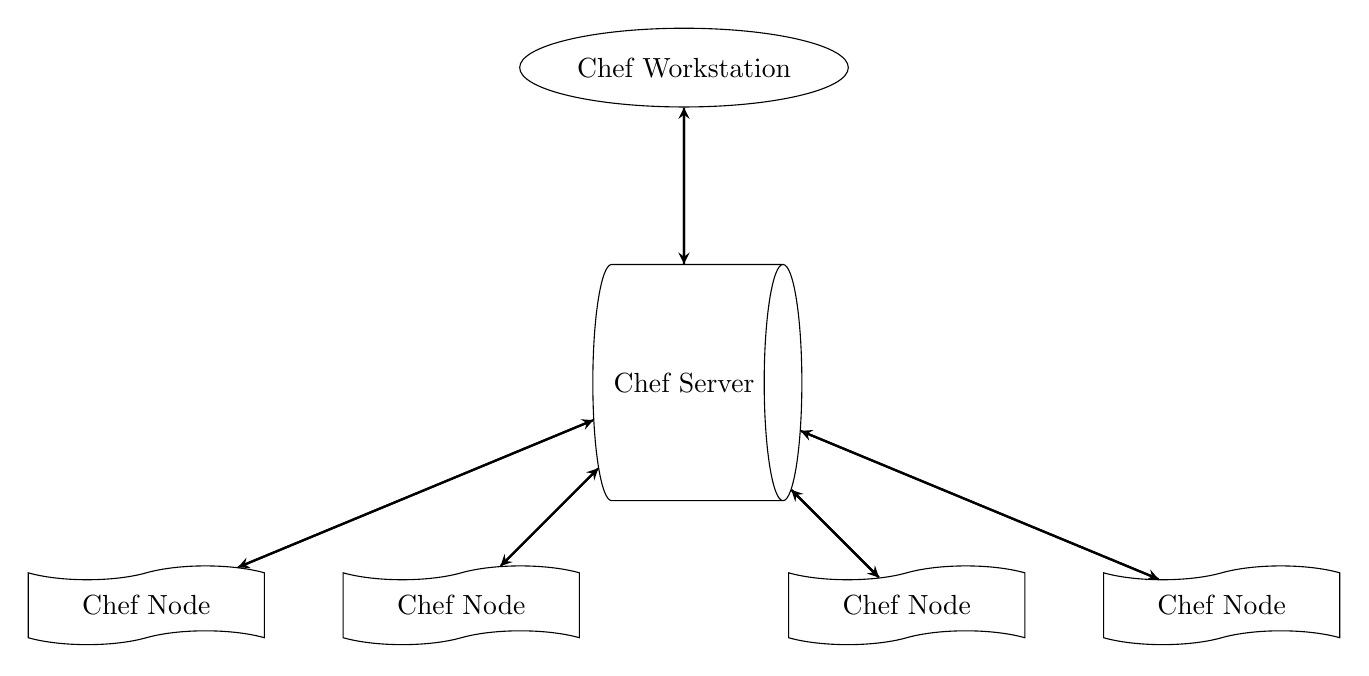
\begin{tikzpicture}[node distance=4cm]
\node (workstation) [workstation] {Chef Workstation};
\node (server) [server, below of=workstation] {Chef Server};
\node (cnode_one) [cnode, below left of=server] {Chef Node};
\node (cnode_two) [cnode, below right of=server] {Chef Node};
\node (cnode_three) [cnode, right of=cnode_two] {Chef Node};
\node (cnode_four) [cnode, left of=cnode_one] {Chef Node};

\draw [arrow] (workstation) -- node {} (server);
\draw [arrow] (server) -- node {} (workstation);

\draw [arrow] (cnode_one) -- node {} (server);
\draw [arrow] (server) -- node {} (cnode_one);
\draw [arrow] (cnode_two) -- node {} (server);
\draw [arrow] (server) -- node {} (cnode_two);
\draw [arrow] (cnode_three) -- node {} (server);
\draw [arrow] (server) -- node {} (cnode_three);
\draw [arrow] (cnode_four) -- node {} (server);
\draw [arrow] (server) -- node {} (cnode_four);

\end{tikzpicture}
\end{center}

\subsection{Features}
Chef provides the following features:
\begin{itemize}
\item
Automatic Backup
\item
Automatic Notifications
\item
Compliance Management
\item
Configuration Management
\item
Data Recovery
\item
Data Visualization
\item
Real Time Analytics
\item
Real Time Data
\item
Real Time Monitoring
\item
Real Time Notifications
\item
Real Time Reporting
\item
Real Time Updates
\item
Server Monitoring

\end{itemize}

\subsection{Official Website}
The official website for Chef is located at \href{https://www.chef.io}{https://www.chef.io}.
\subsection{Latest Version}
\subsection{Advantages}
\subsection{Disadvantages}

\newpage
\section{Ansible}
\subsection{Components}
\subsection{Architecture}
\subsection{Features}
\subsection{Official Website}
\subsection{Latest Version}
\subsection{Advantages}
\subsection{Disadvantages}

\newpage
\section{Fuel}
\subsection{Components}
\subsection{Architecture}
\subsection{Features}
\subsection{Official Website}
\subsection{Latest Version}
\subsection{Advantages}
\subsection{Disadvantages}

\newpage
\section{Puppet}
\subsection{Components}
\subsection{Architecture}
\subsection{Features}
\subsection{Official Website}
\subsection{Latest Version}
\subsection{Advantages}
\subsection{Disadvantages}

\newpage
\section{Compass}
\subsection{Components}
\subsection{Architecture}
\subsection{Features}
\subsection{Official Website}
\subsection{Latest Version}
\subsection{Advantages}
\subsection{Disadvantages}

\end{document}